\documentclass[ngerman,compress]{beamer}

\mode<presentation>
{
  \useoutertheme[footline=titleinstituteauthor]{c4}
  \useinnertheme{circles}
  \usecolortheme{c4}
  %\setbeamercovered{transparent}
  \setbeamercovered{highly dynamic}
}

\usepackage{babel}
\usepackage[utf8]{luainputenc}
\usepackage{fontspec}
\usepackage{listings}
\usepackage{color}
\usepackage{mathtools}

% Multimedia
%\usepackage{multimedia}

% sets the listings style
\definecolor{sh_comment}{rgb}{0.12, 0.38, 0.18 } %adjusted, in Eclipse: {0.25, 0.42, 0.30 } = #3F6A4D
\definecolor{sh_keyword}{rgb}{0.3, 0.3, 0.875}  % #5F1441
\definecolor{sh_string}{rgb}{0.875, 0.85, 0.11} % #101AF9

\lstset{basicstyle=\tiny\ttfamily,
	showspaces=false,
	showtabs=false,
	showstringspaces=false,
	columns=fullflexible,
	stringstyle=\color{sh_string},
	keywordstyle=\color{sh_keyword}\bfseries,
	commentstyle=\color{sh_comment}\itshape
	}

\title[STM32 - Transistoren, LEDs - u23 2013]
{\textbf{STM32 - Transistoren, LEDs}\\u23 2013}

\author[ike <ike@koeln.ccc.de>]
{andy, florob, gordin, ike, meise, tobix, zakx}

\institute[Chaos Computer Club Cologne]
{
Chaos Computer Club Cologne e.V.\\
http://koeln.ccc.de \\
}

\date{Cologne\\2013-11-18}

\pgfdeclareimage[height=1cm]{barcode}{./c4-logo}
\logo{\pgfuseimage{barcode}}


% Folgendes sollte gelC6scht werden, wenn man nicht am Anfang jedes
% Unterabschnitts die Gliederung nochmal sehen möchte.
%\AtBeginSection[]
%{
%  \begin{frame}<beamer>
%    \frametitle{Gliederung}
%    \tableofcontents[currentsection,currentsubsection]
%  \end{frame}
%}

% Falls Aufzählungen immer schrittweise gezeigt werden sollen, kann
% folgendes Kommando benutzt werden:
%\beamerdefaultoverlayspecification{<+->}


\begin{document}

\begin{frame}
  \titlepage
\end{frame}

\AtBeginSubsection

\begin{frame}
  \tableofcontents
  % Die Option [pausesections] könnte nützlich sein.
\end{frame}



\section{LEDs}


\subsection{Ansteuerung}

\begin{frame}
	\frametitle{Wie funktionieren LEDs?}
	\begin{itemize}
		\item Spannung dran - Licht an
		\item Spannung weg - Licht aus
		\item Ein bisschen komplizierter:
		\item Strom da - Licht an
		\item Strom weg - Licht aus
		\item Viel Strom da - Licht kurz an
	\end{itemize}
\end{frame}

\begin{frame}
	\frametitle{Ansteuerung}
	\begin{itemize}
		\item LEDs verbrauchen eine gewisse Spannung (je nach Farbe)
		\item Brauchen einen gewissen Strom
		\item normalerweise 20 mA
		\item Es gibt auch High / Low Power LEDs
	\end{itemize}
\end{frame}

\begin{frame}
	\frametitle{Ansteuerung}
	\begin{itemize}
		\item Um den Strom einzustellen braucht man einen Vorwiderstand
		\item Den berechnet man mit $U = R * I$:
		\item $V_{cc} = U_R + U_D$
		\item $U_R = I_R * R_R$
		\item $\rightarrow R_R = (V_{cc} - U_D) / I$
	\end{itemize}
	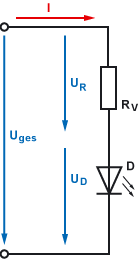
\includegraphics[width=0.8in]{vorwid.png}
\end{frame}

\begin{frame}
	\frametitle{Probleme}
	\begin{itemize}
		\item Die meisten Mikrocontroller können nicht genug Saft abgeben um
			mehrere LEDs zu betreiben
		\item LEDs sind sehr empfindlich gegenüber dem Strom
		\begin{itemize}
			\item Bei kleinem Strom leuchten sie schwach
			\item Bei schon wenig mehr als 20 mA brennen sie durch
		\end{itemize}
		\item Wir werden beide Probleme angehen.
	\end{itemize}
	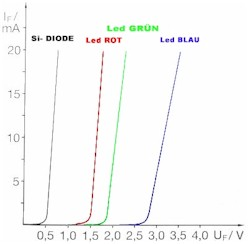
\includegraphics[width=1in]{led.jpg}
\end{frame}


\section{Transitoren}

\subsection{Grundlegende Elektronik}

\begin{frame}
	\frametitle{(Bipolare NPN-) Transistoren}
	\begin{itemize}
		\item Benutzt man als elektronische Schalter
		\item Hauptsächlich sind sie aber Stromverstärker
	\end{itemize}
	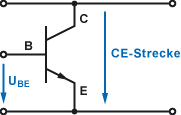
\includegraphics[width=2in]{transistor.png}
	\begin{itemize}
		\item Über CE kann maximal $\beta$ (normalerweise \~ 100) mal so viel
			Strom fließen, wie über BE.
		\item Erste Anwendung: Macht man $I_{BE}$ groß genug, wird $I_{CE}$
			nicht beeinträchtigt $\rightarrow$ elektronischer Schalter.
	\end{itemize}
\end{frame}

\subsection{Anwendungen}

\begin{frame}
	\frametitle{Elektronischer Schalter}
	\begin{itemize}
		\item Beim Schalten (wechseln) ist der Trnasistor kurz in einem
			Überlastbereich
		\item Man will den Steuerstrom \~ 10 mal höher einstellen als benötigt
	\end{itemize}
\end{frame}

\begin{frame}
	\frametitle{Elektronischer Schalter}
	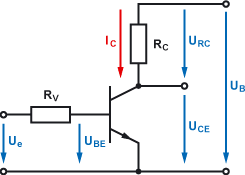
\includegraphics[width=1in]{schalter.png}
	\begin{itemize}
		\item Links: Widerstand stellt den Steuerstrom ein
		\item Rechts: Lastkreis
		\item Basiswiderstand: $R_B = V_{CC} / I_B$
	\end{itemize}
\end{frame}

\begin{frame}
	\frametitle{Dioden}
	\begin{itemize}
		\item Dioden lassen Strom nur in eine Richtung durch
		\item An Dioden fallen immer\footnote{Abhängig vom Material
			(Germanium $0,3V$), Temperatur und natürlich nicht mehr als die angelegte
			Spannung.} $0,7 V$ ab.
	\end{itemize}
	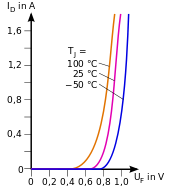
\includegraphics[width=1in]{diod.png}
\end{frame}

\begin{frame}
	\frametitle{Konstantstromquelle 1}
	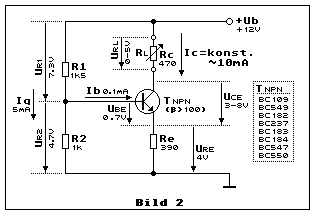
\includegraphics[width=2in]{konst1.png}
	\begin{itemize}
		\item Ziel: Möglichst konstanter Strom, unabhängig vom Verbauch und
			$V_{cc}$
		\item Links: Spannungsteiler
	\end{itemize}
\end{frame}

\begin{frame}
	\frametitle{Konstantstromquelle 2}
	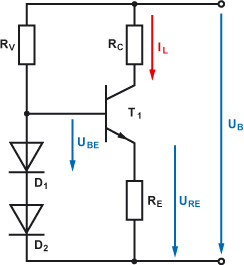
\includegraphics[width=1in]{konst2.png}
	\begin{itemize}
		\item Links: Dioden machen Referenzspannung $1,4 V$
		\item BE wirkt wie eine Diode ($\rightarrow 0,7 V$)
		\item Mit $R_E$ stellt man den Konstantstrom ein:
		\item $I_L = U_{RE} / R_E = 0.7 V / R_E$
		\item Den Querstrom will man etwa 10 mal größer als benötigt haben.
	\end{itemize}
\end{frame}
\end{document}
